%    ----    ----    Q 1    ----    ----

\begin{question}
  Justify the relations $y = y'$ and $z = z'$ of Eq1-1a by symmetry arguments.
\end{question}

\begin{solution}
  Eq1-1a describes the Galilean transformation between the two frames of reference depicted in \figref{fig:1q1}.
  \begin{align*}
    x' &= x - vt \\
    y' &= y \\
    z' &= z
  \end{align*}

  The transformation between $y$ and $y'$ because for $y=y_0$, $y'=y_0$ (see red lines in \figref{fig:1q1}). Similarly for $z$ and $z'$.
\end{solution}

\begin{figure}[h] \centering
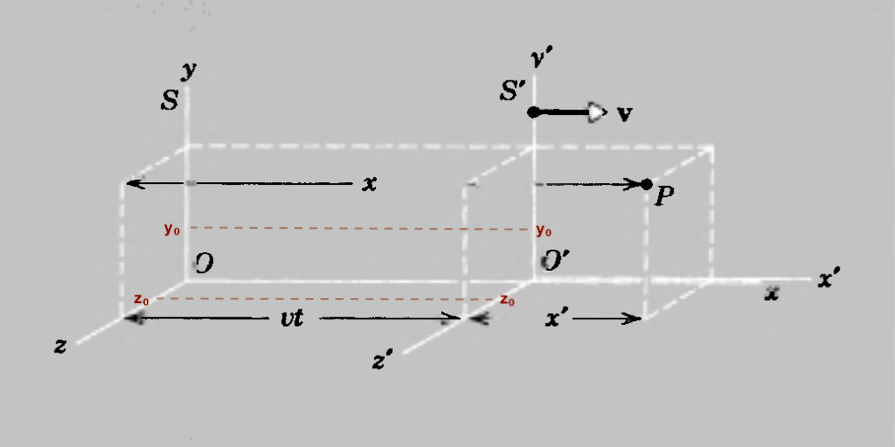
\includegraphics[width=9cm]{fig/1q1.png}
\caption{Resnick's diagram depicting the two inertial frames of reference $S$ and $S'$. $S'$ is moving with velocity $v$ with respect to $S$. Point $P$ is an event, whose space-time coordinates may be measured by each observer.}\label{fig:1q1}
\end{figure}

%    ----    ----    Q 2    ----    ----

\begin{question}
  Momentum is conserved in a collision of two objects as measured by an observer on a uniformly moving train. Show that momentum is also conserved for a ground observer.
\end{question}
\begin{solution}
  Consider two point particles of mass $m_1$ \si{kg} and $m_2$ \si{kg} travelling at speeds $v_1$ \si{m.s^{-1}} and $v_2$ \si{m.s^{-1}} respectively (\figref{fig:1q2}). Take the direction of motion of $v_1$ as being the positive direction. Then the total momentum for an observer inside the train before the collision is

  \begin{equation}
    p = m \cdot v, ~ p_{\text{before}} = m_1 v_1 - m_2 v_2 = p_{\text{after}}
  \end{equation}

  since the question tells us momentum is conserved for an observer inside the train.

  An observer outside the train will see the particles moving at a different speed, namely $v'_1 = v_1 + v_3$ and $- v'_2 = - v_2 + v_3$. Hence,
  \begin{equation} \label{eq:q2eq2}
    p_{\text{before}} = m_1 (v_1 + v_3) + m_2 (- v_2 + v_3) = m_1 v_1 - m_2 v_2 + v_3 (m_1 + m_2)
  \end{equation}
  which is conserved since $m_1 v_1 - m_2 v_2$ is conserved by the assumption, and $v_3$, $m_1$ and $m_2$ are constants.
\end{solution}

\begin{figure}[h] \centering
  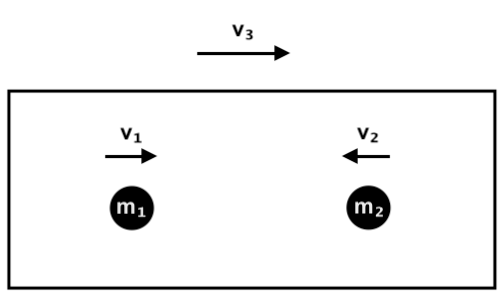
\includegraphics[width=6cm]{fig/1q2.png}
  \caption{Two particles colliding inside a train travelling at velocity $v_3$ \si{m.s^{-1}}.} \label{fig:1q2}
\end{figure}

%    ----    ----    Q 3    ----    ----

\begin{question}
  Repeat Q2 under the assumption that after the collision the masses of the two objects are different from what they were before, that is assume a transfer of mass took place in the course of the collision. Show that for momentum to be conserved for the ground observer, conservation of mass must hold true.
\end{question}

\begin{solution}
  Consider this situation from the point of view of the observer on the train. The two objects are initially moving with velocities and masses $(v_1, m_1)$ and $(-v_2, m_2)$ respectively. After the collision, both their velocities and masses change to $(v_4, m_4)$ and $(v_5, m_5)$ again respectively. Note that $v_4, v_5$ can be positive or negative so we don't need to worry about any negative signs. Then, since again we are told that momentum is conserved, we have:
  \begin{equation}
    p_{\text{before}} = m_1 v_1 - m_2 v_2 = m_4 v_4 + m_5 v_5 = p_{\text{after}}
  \end{equation}

  We still have \eqref{eq:q2eq2} for the total momentum before the collision from the point of view of an outside observer. After the collision, we similarly have
  \begin{equation}
    p_{\text{after}} = m_4 ( v_4 + v_3 ) + m_5 ( v_5 + v_3 ) = m_4 v_4 + m_5 v_5 + v_3 (m_4 + m_5).
  \end{equation}

  From the assumption, we know that $m_1 v_1 - m_2 v_2 = m_4 v_4 + m_5 v_5$, so for momentum to be conserved we must have $m_1 + m_2 = m_4 + m_5$, conservation of mass, as expected. s
\end{solution}

%    ----    ----    Q 4    ----    ----

\begin{question}
  Kinetic energy is conserved in an elastic collision by definition. Show, using the Galilean transformation equations, that if a collision is elastic in one frame of reference then it is ellastic in all intertial frames.
\end{question}
